\chapter{实现细节}


\section{接口层封装}

\subsection{中断向量分配器实现}

为实现3.3.4章节中的中断向量复用,本设计在硬件接口层实现了一个中断向量分配器。

由于硬件中存储了协程id与中断向量号的对应关系,因此软件接口只管理每个中断向量号的使用情况。本设计中,分配器基于32位位图实现。该位图提供基本的方法,如设置位、清除位和查询首个零位。

其中为提高性能,查询首个零位使用Rust内建方法 \verb|trailing_zeros|。该方法返回最低有效零位的索引,在risc-v中可以被映射成CLZ等硬件指令。具体算法如\ref{alg:find_first_unset}所示。

% 查找第一个空闲位的算法

\begin{algorithm}
  \caption{查找位图中首个零位}
  \label{alg:find_first_unset}
  \begin{algorithmic}
    \Function{find\_first\_unset}{bitmap: 32-bit integer}
    \State $inverted \gets \sim bitmap$
    \If{$inverted = 0$}
    \State \Return None
    \Else
    \State \Return trailing\_zeros($\textit{inverted}$)
    \EndIf
    \EndFunction
  \end{algorithmic}
\end{algorithm}

分配器基于上述的位图结构进行封装,提供了初始化、分配、释放接口,实现类图如图\ref{中断向量分配器类图}。

% 中断向量分配器类图
\begin{figure}[htbp]
  \centering
  \includesvg[inkscapelatex=false,width=0.8\textwidth]{images/IrqAllocator}
  \caption{中断向量分配器类图}\label{中断向量分配器类图}
\end{figure}


\subsection{硬件队列封装}

由于内核和用户态的地址空间存在差异,因此分别在用户态和内核态的接口层对\texttt{taic\_driver}进行了不同的封装。

内核中接口层首先定义了TAIC的寄存器物理地址基址、本地队列数量、内核线程id等常量。然后,使用\texttt{lazy\_static}宏声明了一个内核中全局唯一的本地队列\texttt{LOCAL\_QUEUE}。该队列使用常量参数调用\texttt{taic\_driver}中\texttt{alloc\_lq}的方法分配。

接口层提供\texttt{get\_lq}方法返回\texttt{LOCAL\_QUEUE}的Arc智能指针,用于异步运行时就绪队列的初始化。

接口层封装了发送者和接收者的注册逻辑。

其中\texttt{register\_sender}用于将内核的队列的注册成为另一个全局队列的消息发送方。该方法直接调用\texttt{LOCAL\_QUEUE}中的\texttt{register\_sender}方法,并固定\texttt{os\_id}参数为常量。

其中\texttt{register\_receiver}用于将内核的队列的注册成为另一个全局队列的消息接受方。该方法将设置了两个布尔变量:preempt与reusable分别表示该次注册是否抢占之前的注册以及是否可循环使用。接收方 ID、可抢占性与可复用性被按位编码为一个 \texttt{handler} 值,并传递给 \texttt{LOCAL\_QUEUE} 的 \texttt{register\_receiver} 方法完成注册。

接口层还提供\texttt{send\_signal}方法,用于向其他队列发送信号,通过中断向量唤醒对方队列中的协程。

用户态的接口层中,使用\texttt{thread\_local}宏定义了线程局部变量\texttt{LQ\_MANAGER}。该变量作为硬件资源的全局管理实例,整合了中断向量分配器以及全局队列。用户态的接口中使用\texttt{LQ\_MANAGER}中的队列代替全局队列,实现了硬件资源的线程隔离。

\section{缓冲区优化}

\subsection{IPC消息字段修改}

为了在通信时附带协程所申请的中断向量信息,本设计在\texttt{IPC\_Item}中新增了vec字段用于指示发送消息的协程的中断向量。若该字段为0,则表明该协程无中断向量,需通过\texttt{dispatcher}协程唤醒。

% ipcitem位域图
\begin{figure}[htbp]
  \centering
  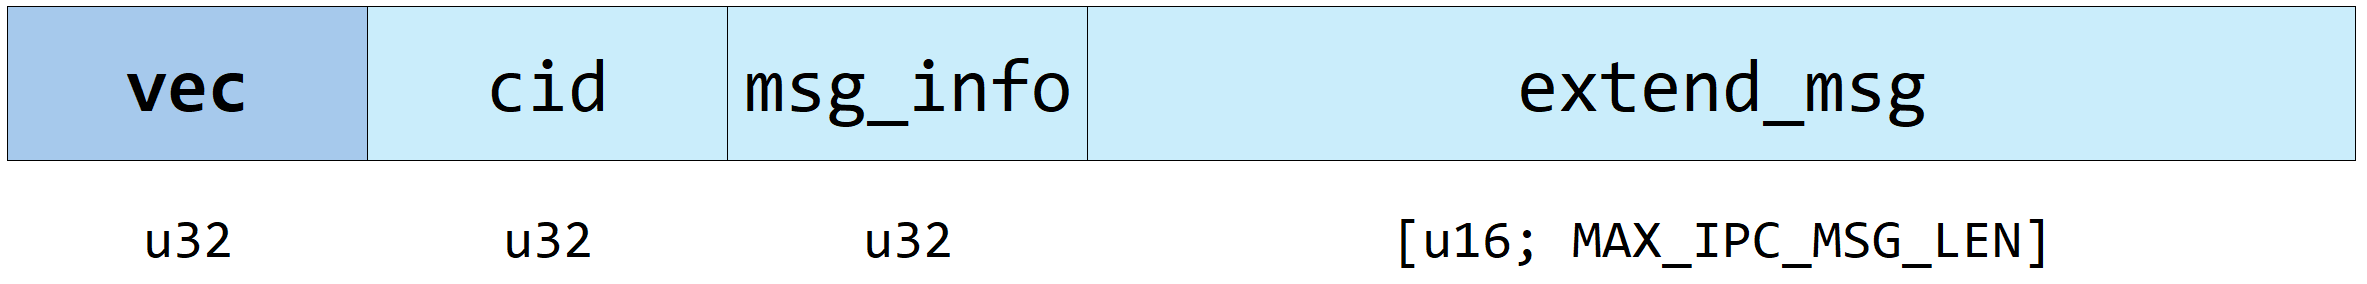
\includegraphics[width=0.8\textwidth]{images/ipc_item.png}
  \caption{ipcitem结构}\label{ipc_item结构}
\end{figure}

\subsection{环形队列结构优化}

依据\ref{sec:buffer}中的设计,缓冲区实现如图\ref{缓冲区类图}所示。

\begin{figure}[htbp]
  \centering
  \includesvg[inkscapelatex=false,width=\textwidth]{images/newbuffer}
  \caption{缓冲区类图}\label{缓冲区类图}
\end{figure}

缓冲区中\texttt{data}为数据区,由长度为4096的\texttt{ipc\_item}数组实现,用于存储调用时的传递消息。

\texttt{req\_items}和\texttt{res\_items}分别为请求消息与回复消息的索引队列,两者均采用\texttt{ItemsIdxQueue}数据结构实现。\texttt{ItemsIdxQueue}基于\texttt{SafeRingBuffer}封装,实现了一个线程安全的环形队列,提供了入队\texttt{write\_free\_idx}和出队\texttt{get\_first\_idx}两个基础方法。
\texttt{SafeRingBuffer}是一个无锁环形缓冲区,其内部使用原子变量\texttt{count}记录缓冲区中有效元素的数量,以此保证安全的读写。

\texttt{recv\_req\_status}和\texttt{recv\_reply\_status}为两个布尔类型的原子变量,分别表示接受请求的协程的当前状态与接受回复的\texttt{dispatcher}协程的当前状态。这两个状态标志减少了唤醒的次数,避免了重复调度。

\texttt{idx\_allocator}为数据区存储空间的索引分配器,负责管理数据区索引号的分配与回收,其内部同样使用位图实现。

缓冲区索引号的分配仅由用户态线程发起,而内核中的处理协程始终使用相同的索引号进行回复。因此,缓冲区的索引号总是由同一线程进行分配,具有天然的线程安全性。同时,两个环形队列的通过原子变量实现了并发访问控制,整个缓冲区在多线程环境下可实现无锁并发访问。该设计降低了因分配器引入导致的性能开销,使分配回收操作在极短的时间内即可完成,确保了高并发场景下的稳定性与效率。

\section{执行器硬件适配}

为了使异步运行时能够调用硬件能力,本设计对内核中异步运行时的执行器\texttt{Executor}中部分数据结构与方法进行了重写。

因为缓冲区的逻辑优化,已不再需要进行消息转发,因此本设计删除了相关变量,并将原有的就绪队列改为TAIC中队列的Arc引用\texttt{Arc<LocalQueue>}。在异步运行时初始化时,会调用下层的接口层代码,申请一个就绪队列,并将其引用传给执行器完成就绪队列的初始化。

\texttt{spawn}为执行器的协程生成方法。在该方法中,\texttt{Executor}使用TAIC提供的\texttt{task\_enqueue}方法将生成的协程加入就绪队列。因为TAIC句柄的第一位和第二位用作重复注册和抢占的标志位,因此调用该方法时需要协程id左移2位。

\texttt{fetch}为执行器从就绪队列中调度协程执行的方法。在该方法中使用TAIC提供的\texttt{task\_dequeue}方法取出就绪队列中的就绪协程。


\section{异步系统调用注册}

为实现上述修改,本设计修改了原有的异步系统调用注册相关代码。原有的实现中,异步系统调用注册时会对注册方的相关能力进行检查,并根据调用方生成一个用于处理异步系统调用的协程。本设计中删除了用户态中断的部分逻辑,增加了生成协程时硬件能力注册的代码。


\section{用户接口封装}

\subsection{进程初始化}

为使用户态进程支持异步系统调用能力,系统需要在创建进程时准备相关数据结构,完成异步系统调用的初始化。

\begin{figure}[htbp]
  \centering
  \includesvg[inkscapelatex=false,width=\textwidth]{images/initsyscall}
  \caption{线程初始化异步系统调用时序图}\label{initsyscall}
\end{figure}

该过程时序如图\ref{initsyscall}所示。系统首先需要对异步运行时进行初始化,然后对初始化TAIC的硬件能力。再此过程中,会将TAIC的读写寄存器映射到用户态地址空间。然后对该进程分配接受内核回复通知的能力。基于该通知,利用TAIC的\texttt{alloc\_receiver}函数为进程分配一个队列。接着会为进程初始化一个异步通信的缓冲区,将该缓冲区注册用于异步系统调用,并访问缓冲区的能力。然后,基于通知能力,进行系统调用,进行3.2所述的异步系统调用注册。在注册成功后,利用接口层的\texttt{register\_sender}函数,将当前进程的TAIC队列注册成为系统内核全局队列信号的发送者。最后,调用异步运行时的接口,生产用于中断向量不足时间接唤醒的分发协程。


\subsection{异步系统调用发送协程}

使用该系统的用户可利用异步运行时,生成协程发起异步系统调用。目前给出可能的协程内进行异步系统调用的方法。

协程首先应调用结构层的\texttt{alloc\_vec}函数尝试申请分配一个vec。若分配成功,则利用该vec,调用\texttt{register\_receiver}注册函数将本协程注册成消息的接受者。然后即可通过异步系统调用接口进行异步系统调用。在调用完成后,应释放分配的vec。

该部分算法伪代码如\ref{client_call}:

\begin{algorithm}
  \caption{Client Async SysCall}\label{alg:client_call}
  \begin{algorithmic}
    \Procedure{client\_call\_test}{sender\_id, msg}
    \State \textbf{unsafe}
    \State $cid \gets$ \Call{coroutine\_get\_current}{}
    \State $vec \gets$
    \If {\Call{alloc\_vec}{} \textbf{returns} Some($res$)}
    \State \Call{register\_receiver}{sender\_id, res, cid, true, true}
    \State $res$
    \Else
    \State $0$
    \EndIf
    \For {$i = 0$ \textbf{to} ${call\_cnt} - 1$}
    \State $reply \gets$ \Call{riscv\_Page\_Map}{vec, args} \Comment{await}
    \If {$reply$ \textbf{is Ok}}
    \State \Call{cope}{$reply$}
    \Else
    \State \Call{panic}{``client test fail!''}
    \EndIf
    \EndFor
    \State \Call{free\_vec}{vec}
    \EndProcedure
  \end{algorithmic}
\end{algorithm}


\subsection{异步系统调用接口}

为方便用户使用异步系统调用,异步库提供异步系统调用接口,异步系统调用进行封装。该类接口中会对参数进行编码转换,构造成异步系统调用消息。最后调用\ref{sec:asynccallfunc}中的异步call函数进行异步调用。ReL4中异步系统调用的接口函数如表\ref{syscalltable}所示。

\begin{table}[htb]
  \centering
  \caption{ReL4 异步系统调用表}\label{syscalltable}
  \begin{tabular}{@{}ll@{}}
    \toprule
    \textbf{系统调用}                               & \textbf{功能描述}                  \\
    \midrule
    \texttt{syscall\_untyped\_retype}           & 将未初始化对象重新类型化为指定内核对象类型。         \\
    \texttt{syscall\_riscv\_page\_get\_address} & 获取虚拟页对应的物理地址。                  \\
    \texttt{syscall\_putchar}                   & 向控制台输出单个字符。                    \\
    \texttt{syscall\_putstring}                 & 向控制台输出字符串。                     \\
    \texttt{syscall\_tcb\_bind\_notification}   & 将通知对象绑定到指定的 TCB 上。             \\
    \texttt{syscall\_tcb\_unbind\_notification} & 从 TCB 上解绑通知对象。                 \\
    \texttt{syscall\_cnode\_copy}               & 拷贝 capability 到另一个 cnode 中。    \\
    \texttt{syscall\_cnode\_delete}             & 删除 cnode 中的 capability。        \\
    \texttt{syscall\_cnode\_mint}               & 复制并设置新的权限与 badge 的 capability。 \\
    \texttt{syscall\_riscv\_page\_map}          & 映射物理页到虚拟地址空间。                  \\
    \texttt{syscall\_riscv\_page\_unmap}        & 解除物理页的虚拟映射。                    \\
    \texttt{syscall\_riscv\_pagetable\_map}     & 映射页表到虚拟地址空间。                   \\
    \texttt{syscall\_riscv\_pagetable\_unmap}   & 解除页表映射。                        \\
    \bottomrule
  \end{tabular}
\end{table}

本设计对ReL4中原有接口的封装进行了微小改动,加入了中断向量参数的构造与传递,修改了系统调用接口的常量参数。

\subsection{异步call函数}\label{sec:asynccallfunc}

\texttt{seL4\_call\_with\_item}为发起异步系统调用的关键函数。该函数接受三个参数:接收方id,中断向量以及进程间通信条目,可对目标发起异步的\texttt{sel4\_call}调用。在接收方为0号的异步系统调用中,会调用通知对象的send能力,对系统中处理异步系统调用的端点发送消息,并等待reply回复。

该方法首先获取接受方的异步通信缓冲区,然后向缓冲区申请id。成功申请到id后,依据传入的消息参数将消息写入缓冲区。此时,会检测冲区中的原子变量\texttt{recv\_req\_status}。若原子变量为\texttt{false},则说明内核中的处理协程已经因空闲阻塞。此时会先调整原子变量的值,防止并发时重复唤醒。然后调用接口层中的\texttt{send\_signal}方法像内核发送信号,唤醒对应协程。完成操作后,该方法会在此阻塞,等待内核的回复。当协程因收到回复而被再次调度执行时,会依据先前的缓冲区id获取回复消息并进行返回。

该方法的伪代码如下所示:

\begin{algorithm}
  \caption{\texttt{sel4\_call\_with\_item(recv, vec, item)}}
  \begin{algorithmic}[0]  % 关闭行号
    \State buffer $\gets$ try get mutable buffer from \texttt{SENDER\_MAP[*recv]}
    \If{buffer is None}
    \State \Return \texttt{Err("Failed to get service buffer")} \Comment 获取失败
    \EndIf

    \State idx $\gets$ buffer.idx\_allocator.allocate()
    \If{idx is None}
    \State \Return \texttt{Err("Failed to allocate index in buffer")} \Comment 索引分配失败
    \EndIf

    \State buffer.data[idx] $\gets$ *item
    \If{buffer.req\_items.write\_free\_idx(idx) is Err}
    \State \Return \texttt{Err("Failed to write free index")} \Comment 写入请求队列失败
    \EndIf

    \If{buffer.recv\_req\_status.load() == false}
    \State buffer.recv\_req\_status.store(true)
    \State send\_signal(*recv, vec) \Comment 唤醒接收方
    \State \texttt{TEST\_TAIC\_SEND\_SIGNAL += 1}
    \EndIf

    \State yield\_now().await \Comment 阻塞等待响应
    \State buffer.idx\_allocator.release(idx) \Comment 释放索引
    \State \Return \texttt{Ok(buffer.data[idx])}
  \end{algorithmic}
\end{algorithm}

\subsection{分发协程}
当中断向量不足,需要分发协程进行唤醒的软件转发。异步库提供该协程的实现:

该协程相当于接收回复消息的服务端。协程首先会从参数中解析出异步系统调用的缓冲区,然后将自身注册成为0号中断向量的接收者,然后会进入主循环。在循环内部,该协程不断从缓冲区的“接受回复索引队列”中取出需要唤醒的消息id。如果成功取到,则会根据消息中的协程id,通过\texttt{coroutine\_wake}接口唤醒对应的协程。如果队列为空,则会调整缓冲区中表示自身状态的原子变量
\texttt{recv\_reply\_status},然后调用\texttt{yield\_now}接口阻塞自身,让出执行权。

\section{内核处理算法}

内核中异步系统调用的处理协程相当于内核中的服务端,与分发协程类似。该协程会在异步系统调用注册时生成,并通过参数传递得到缓冲区能力。协程解析出缓冲区后,即进入主循环处理消息。

在主循环中,协程尝试从缓冲区的\texttt{req\_items}索引队列中获取消息索引。如果成功获取到消息,则解析消息中的标签,根据不同的系统调用进行不同的处理。处理完成红,会根据消息索引将处理的结果写回缓冲区。如果请求消息中的中断向量为0,则直接通过硬件接口\texttt{send\_signal}发送信号唤醒原协程。否则,会先将回复消息的索引写入队列\texttt{res\_items},然后根据缓冲区中的原子变量\texttt{recv\_reply\_status}判断分发协程的状态。若分发协程已经阻塞,则通过\texttt{send\_signal}接口唤醒分发协程。

当缓冲区中所有消息都被处理完毕后,协程会调用\texttt{yield\_now}接口阻塞自身,等待唤醒。

该部分算法的伪代码如算法\ref*{alg:async_syscall_handler}所示:

\begin{algorithm}[!h]
  \caption{异步系统调用处理协程 \texttt{async\_syscall\_handler}}\label{alg:async_syscall_handler}
\begin{algorithmic}
\Function{async\_syscall\_handler}{$process\_id$, $tcb$}
    \State $new\_buffer \gets$ \Call{convert\_to\_mut\_type\_ref}{$new\_buffer\_cap$}
    \Loop
        \If{\Call{has\_request\_item}{$new\_buffer$}}
            \State $idx \gets$ \Call{get\_first\_idx}{$new\_buffer.req\_items$}
            \State $item \gets$ \Call{deep\_copy}{$new\_buffer.data[idx]$}
            \State $label \gets$ \Call{AsyncMessageLabel::from}{$item.msg\_info$}
            \State \Call{debug}{"handle async syscall: \{label\}"}
            \State $reply \gets$ \Call{handle\_syscall}{$label$, $item$}
            \State $new\_buffer.data[idx] \gets item$
            \If{$item.vec \neq 0$}
                \State \Call{send\_signal}{$process\_id$, $item.vec$}
            \Else
                \State \Call{release\_buffer\_item}{$new\_buffer$, $idx$}
                \If{\Call{recv\_reply\_status}{$new\_buffer$} is false}
                    \State \Call{set\_recv\_reply\_status}{$new\_buffer$, true}
                    \State \Call{send\_signal}{$process\_id$, 0}
                \EndIf
            \EndIf
        \Else
            \State \Call{set\_recv\_req\_status}{$new\_buffer$, false}
            \State \Call{yield\_now}{} \Comment{Block until next notification}
        \EndIf
    \EndLoop
\EndFunction
\end{algorithmic}
\end{algorithm}



\section{本章小结}

本章详细介绍了支持异步系统调用的系统关键实现细节。首先,通过中断向量分配器的设计,实现了协程与硬件中断之间的高效映射,使用基于位图的分配结构以及硬件友好的算法,提升了分配性能。随后,在接口层对内核与用户态的硬件队列进行了合理封装,分别实现了局部队列的独立管理与中断驱动的异步唤醒机制。

在缓冲区部分,针对高并发场景进行了深度优化。通过双环形队列配合原子状态变量,确保了消息队列的无锁并发访问能力,同时减少了不必要的线程唤醒,有效提升了运行效率。缓冲区索引的线程安全性也通过线程唯一分配策略得以保证。

针对执行器模块,本设计完成了其与硬件异步能力的适配,替换了原有就绪队列逻辑,并引入基于TAIC队列的协程调度机制,形成软硬协同的调度执行路径。此外,为适配上述机制,对异步系统调用的注册、发起、接收、回复及中断转发等环节进行了系统性重构。

最后,完整实现了服务端处理协程与客户端分发逻辑,为异步系统调用提供了完整的数据路径和调度保障,确保异步系统调用在用户态与内核态间的高效传输与响应。通过本章的设计与实现,整个系统的异步通信能力得以构建,为后续章节的性能评估与应用部署奠定基础。